% !TeX spellcheck = cs_CZ
%{\tikzset{external/prefix={tikz/FYZII/}}
% \tikzset{external/figure name/.add={ch26_}{}}
%---------------------------------------------------------------------------------------------------
% file fey2ch26.tex
%---------------------------------------------------------------------------------------------------
%=========================== Kapitola Lorentzovy transformace polí =================================
\setchaptertoc
\chapter{Lorentzovy transformace polí}\label{fyz:IIchapXXVI}

  \section{Čtyřpotenciál pohybujícího se náboje}\label{fyz:IIchapXXVIsecI}
  \section{Pole bodového náboje pohybující se konstantní 
  rychlostí}\label{fyz:IIchapXXVIsecII}
  \section{Relativistické transformace polí}\label{fyz:IIchapXXVIsecIII}
  \section{Pohybové rovnice v relativistickém označení}\label{fyz:IIchapXXVIsecIV}
  \section{Příklady a cvičení}\label{fyz:IIchapXXVIsecV}



    \begin{figure}[ht!] %\ref{fyz:fig602}
      \centering
      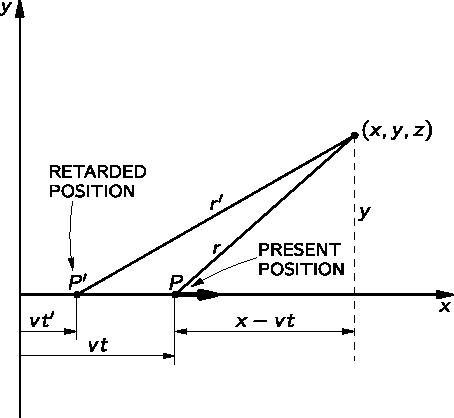
\includegraphics[width=0.7\linewidth]{fyz_fig602.pdf}
      \caption{
               (\cite[s.~707]{Feynman02})}
      \label{fyz:fig602}
    \end{figure}

    \begin{figure}[ht!] %\ref{fyz:fig603}
      \centering
      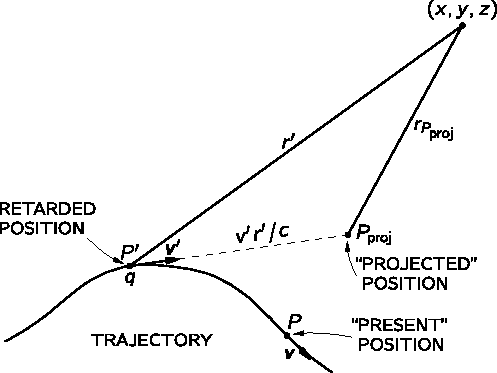
\includegraphics[width=0.7\linewidth]{fyz_fig603.pdf}
      \caption{
               (\cite[s.~707]{Feynman02})}
      \label{fyz:fig603}
    \end{figure}

    \begin{figure}[ht!] %\ref{fyz:fig604}
      \centering
      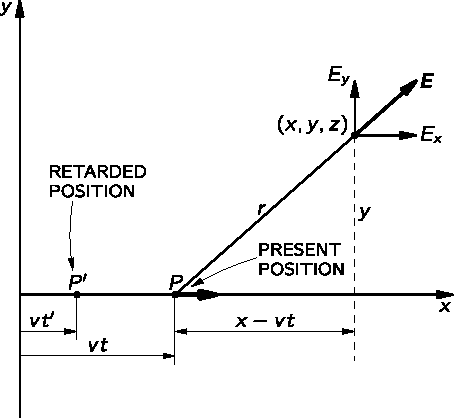
\includegraphics[width=0.7\linewidth]{fyz_fig604.pdf}
      \caption{
               (\cite[s.~707]{Feynman02})}
      \label{fyz:fig604}
    \end{figure}

    \begin{figure}[ht!] %\ref{fyz:fig605}
      \centering
      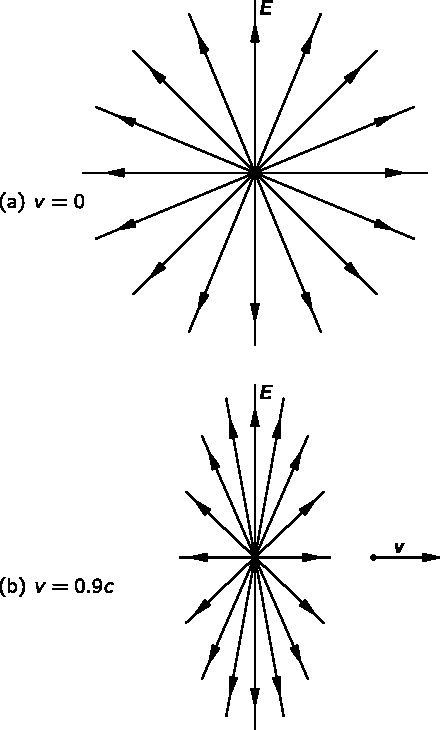
\includegraphics[width=0.7\linewidth]{fyz_fig605.pdf}
      \caption{
               (\cite[s.~707]{Feynman02})}
      \label{fyz:fig605}
    \end{figure}

    \begin{figure}[ht!] %\ref{fyz:fig606}
      \centering
      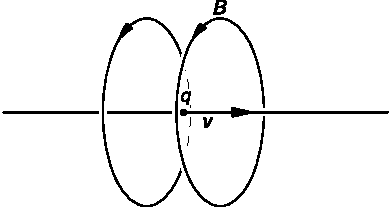
\includegraphics[width=0.7\linewidth]{fyz_fig606.pdf}
      \caption{
               (\cite[s.~707]{Feynman02})}
      \label{fyz:fig606}
    \end{figure}

    \begin{figure}[ht!] %\ref{fyz:fig607}
      \centering
      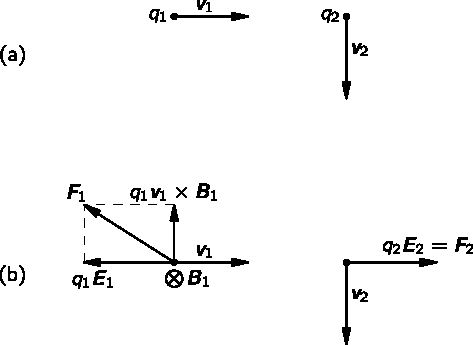
\includegraphics[width=0.7\linewidth]{fyz_fig607.pdf}
      \caption{
               (\cite[s.~707]{Feynman02})}
      \label{fyz:fig607}
    \end{figure}

    \begin{figure}[ht!] %\ref{fyz:fig608}
      \centering
      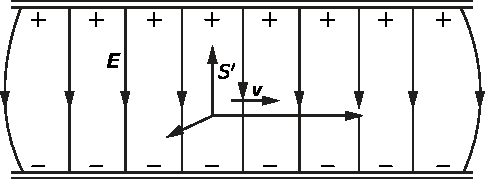
\includegraphics[width=0.7\linewidth]{fyz_fig608.pdf}
      \caption{
               (\cite[s.~707]{Feynman02})}
      \label{fyz:fig608}
    \end{figure}

    \todo[inline]{Kapitola fey2ch26 je nedodělaná, obsahuje pouze obrázky}
%} %tikzset
%---------------------------------------------------------------------------------------------------